\documentclass{article}
\usepackage[utf8]{inputenc}
\usepackage[T1]{fontenc}
\usepackage[dutch]{babel}
\usepackage[square,sort,comma,numbers]{natbib}
\usepackage[hyphens]{url}
\usepackage{hyperref}
\setlength
{\parindent}
{0pt}
\setlength
{\parskip}
{1.5ex plus 0.5ex minus 0.2ex}
\usepackage[margin=3.5cm]{geometry}


\title{Gegevensstructuren en Algoritmen: Practicum 3}
\author{Mathias Van Herreweghe - r0456156}
\date{30 mei 2014}

\usepackage{natbib}
\usepackage{graphicx}

\begin{document}

\maketitle
\newpage
\section{Introductie}
Het Image Compositing algoritme is een algoritme dat twee afbeeldingen samenvoegt, dit met een zo klein mogelijk zichtbaar verschil tussen de twee afbeeldingen. Des te minder de grens tussen de twee afbeeldingen opvalt, des te beter het algoritme.

Om dit te realiseren zijn er twee fundamentele algoritmes nodig; seam() en floodfill().
Seam() zal de grens bepalen tussen de twee afbeeldingen en maakt gebruik van Dijkstra's kortste-pad algoritme in combinatie met een binary heap om de grens zo min mogelijk zichtbaar te maken.
Floodfill() zal dan weer de nieuwe afbeeldingen invullen met de oorspronkelijke afbeeldingen rekening houdende met de gevonden grens in seam().
Samen kunnen deze twee algoritmes twee afbeeldingen als het ware aan elkaar 'naaien'.

\newpage
\section{Grafe voor gegeven afbeeldingen}
Betreffende afbeeldingen vindt je hieronder.

\begin{tabular}{| c | c | c |}
\hline
 (7,0,0) & (0,1,0) & (0,0,1) \\
  \hline
 (2,0,0) & (0,8,0) & (0,0,5) \\
  \hline
  (1,0,0) & (0,1,0) & (0,0,8) \\
  \hline
\end{tabular}

\begin{tabular}{| c | c | c |}
\hline
 (0,0,0) & (0,0,0) & (0,0,0) \\
  \hline
 (0,0,0) & (0,0,0) & (0,0,0) \\
  \hline
  (0,0,0) & (0,0,0) & (0,0,0) \\
  \hline
\end{tabular}

Om de figuur van de grafen te verduidelijken geef ik de pixels van de resulterende afbeeldingen de volgende namen, de kleurafstand tussen de twee gegeven afbeeldingen vindt je terug in de haakjes achter elke naam.

\begin{tabular}{| c | c | c |}
\hline
  A(49) & B(1) & C(1) \\
  \hline
  D(4) & E(64) & F(25) \\
  \hline
  G(1) & H(1)& I(64) \\
  \hline
\end{tabular}

\begin{figure}[h!]
\centering
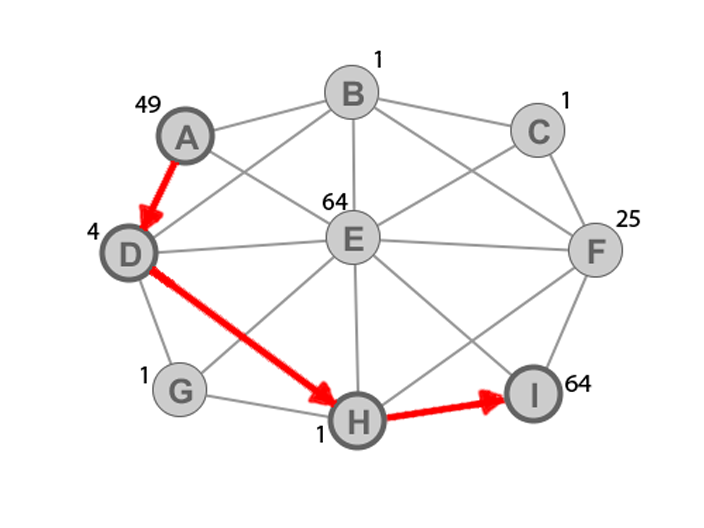
\includegraphics[scale=0.4]{graph.png}
\caption{Grafe met het kortste pad aangeduid in een rode kleur}
\label{fig:Graph}
\end{figure}


\newpage
\section{Alternatieve kleurafstand-formule}

Oorspronkelijke kleurafstand-formule: $ r^2 + g^2 + b^2 $ \newline
Alternatieve kleurafstand-formule: $ \sqrt{r^2 + g^2} $

Afbeeldingen zullen in de praktijk bijna altijd sneller omgezet worden, dit is omdat er met één kleur minder rekening gehouden moet worden, dit leidt tot een rechtstreekser, korter, naïever en dus sneller pad.
Hoe belangrijker blauw zou zijn voor de grens van een nieuwe afbeelding, des te meer posities er versimpeld kunnen worden met slechts twee kleur-waardes. Dus zal bijgevolg de kleurafstand-formule voor de grens lager zijn dan indien men wel met blauw had rekening gehouden. Zo krijg je voor volgende afbeeldingen met de oorspronkelijke kleurafstand-formule een afstand van 10.814, met de alternatieve formule bekomen we slechts een afstand van 7822.

Merk wel op dat men doordat de grens verandert (lees: versimpelt), de resulterende afbeelding er ook anders uit zal zien.

\begin{figure}[h!]
\centering
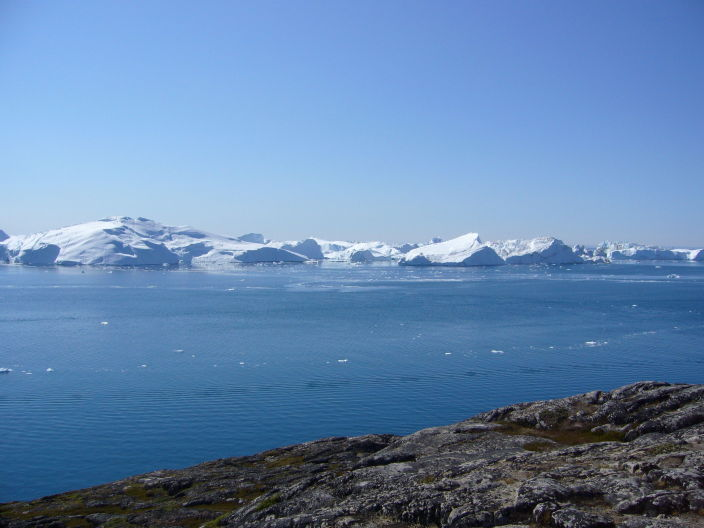
\includegraphics[scale=0.2]{zee1.png}
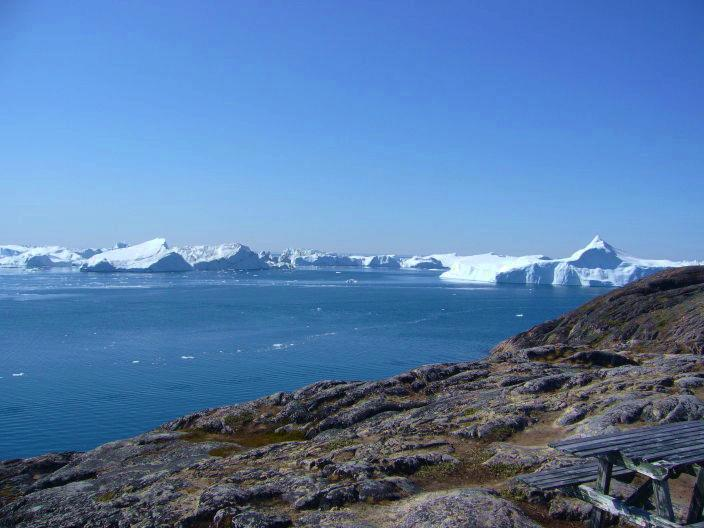
\includegraphics[scale=0.2]{zee2.png}
\caption{zee1.png en zee2.png}
\label{fig:Zee}
\end{figure}

Noemenswaardig is ook dat als men blauw wegneemt uit de formule, afbeelden die -behalve een zwarte scheidingslijn\footnote{Dit is omdat zwart een waarde heeft van rgb(0,0,0) en dus een zwaarte heeft gelijk aan 0, daarbovenop zou de zwaarte telkens 0 zijn indien de scheidingslijn met eender welke kleur op exact dezelfde plaats zou liggen op beide afbeeldingen. Want het verschil tussen de kleur is dan 0.}- volledig uit blauw-waarden bestaan onmogelijk correct samengevoegd kunnen worden. Dit is omdat er zo nooit een correct korstste pad kan berekend worden met Dijkstra's kortste pad algoritme. Dit omdat alle grafes even zwaar zullen zijn\footnote{Namelijk gelijk aan 0.}, alle mogelijke paden bijgevolg dus ook. Zo heeft de achtergrond van blue1.png de kleur rgb(0, 0, 255) en blue2.png de kleur rgb(0, 0, 120). Bij het resultaat zie je duidelijk dat het algoritme geen correcte uitkomst kan vinden.

\begin{figure}[h!]
\centering
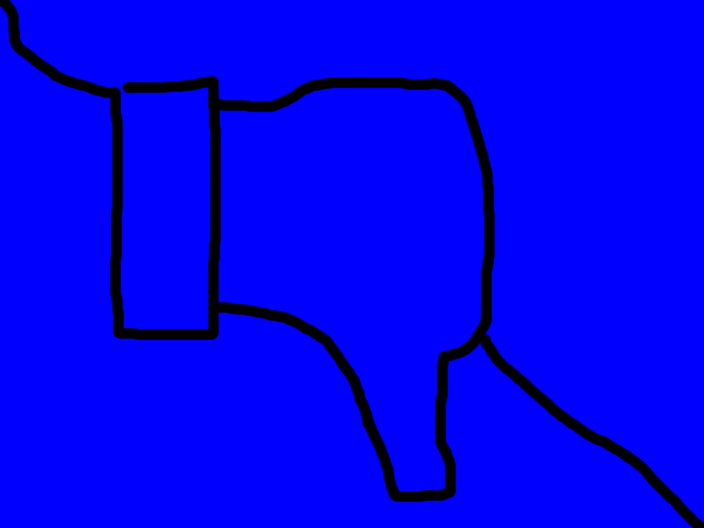
\includegraphics[scale=0.17]{blue1.png}
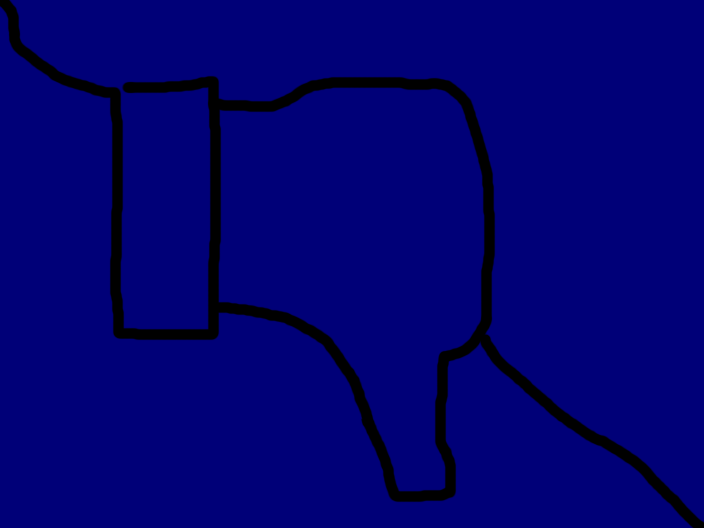
\includegraphics[scale=0.17]{blue2.png}
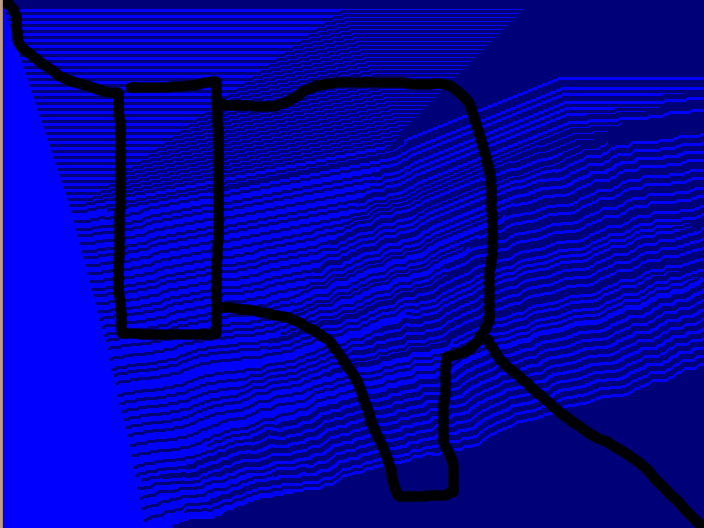
\includegraphics[scale=0.17]{blue-out.png}
\caption{blue1.png, blue2.png en blue-out-incorrect.png}
\label{fig:Blue}
\end{figure}

\section{Afbeelding op harde schijf}

Een mogelijkheid zou zijn om de matrixen op te slaan op de harde schijf door ze in een tekstbestand te schrijven, gevisualiseerd zoals een echte matrix, met vierkantje haakjes rond de waarden, schrijven en lezen naar en van bestanden kan met de hulp van bestaande Java klassen zoals PrintWriter, FileOutputStream, BufferedWriter, OutputStreamWriter, ... Vervolgens zou je via loops tot aan een bepaalde index kunnen komen en deze uitlezen en/of aanpassen. Dit zou echter heel veel tijd in beslag nemen aangezien je telkens alle lijnen en kolommen moet overlopen tot je aan een bepaalde index komt.

Een beter alternatief zou zijn om de gehele matrix te lineariseren en deze op te slaan in een databank op de harde schijf, zij het een SQL database, MongoDB of een andere. Op deze manier kan je queries gebruiken om op de entry van een bepaalde identifier (= gelineariseerde index) te komen en deze vervolgens in te lezen en/of aan te passen. Om dit te verwezenlijken kan je API's gebruiken bedoeld voor deze databanken, voor SQL zou je zo het pakket java.sql\cite{javasql} kunnen gebruiken.

\section{Best-case tijdscomplexiteit}

We splitsen dit op in verschillende delen om het geheel te verduidelijken.
Stel we nemen N is gelijk aan de breedte van de afbeelding vermenigvuldigd met de hoogte. $ N = breedte * hoogte $

De best-case tijdscomplexiteit zal men bekomen indien het kortste pad diagonaal loopt over de afbeeldingen, van linksboven, naar rechtsonder. De lengte van het pad zal als bijgevolg $ \sqrt{breedte^2 + hoogte^2} $ zijn. Dit is het kortst mogelijke pad van linksboven naar rechtsonder.

Ten eerste wordt de methode seam() opgeroepen. Deze zal voor elke pixel zijn buren (meestal 8) een edge toevoegen aan een grafe. We bekomen dus al $ 8 * N $. Vervolgens zal het Dijkstra algoritme het kortste pad berekenen, hetgeen $ (E + V) * log (V) $ tijd neemt in het beste geval, dit zou hoger zijn moesten we een rij of gelinkte lijst zouden gebruiken als data structuur voor Dijkstra. Aangezien er $ E = N * 8 $ edges zullen zijn, en $ V = E * 8 $ vertices, kunnen we dit omzetten naar $ ((8 * N) + (64 * N)) * log (64 * N) = 72 * N * log ( 64 * N) $. Nadien wordt dit kortste pad nog toegevoegd aan een lijst van posities door van elke edge van dit kortste pad de positie toe te voegen. Aangezien het best-case is zullen er zo $ \sqrt{breedte^2 + hoogte^2} $ edges zijn. Dit geeft een totale best-case tijdscomplexiteit van $ 8 * N + 72 * N * log ( 64 * N) + \sqrt{breedte^2 + hoogte^2} $ voor seam().

Voor floodfill() geldt dan weer dat elke pixel die niet tot de naad behoort eenmaal benaderd zal worden. Dit neemt dus $ N - \sqrt{breedte^2 + hoogte^2} $ tijd in beslag. Er worden niet meer dan N pixels onderzocht omdat er eerst gecontroleerd wordt of de betreffende pixel reeds geïnitialiseerd is. Indien dit het geval is wordt het vul-gedeelte overgeslagen en wordt de volgende pixel onderzocht.

Als je deze twee methodes combineert krijg je een tijdscomplexiteit van $ 8 * N + 72 * N * log (64 * N) + \sqrt{breedte^2 + hoogte^2}  +  N - \sqrt{breedte^2 + hoogte^2} = 7 * N + 72 * N * log (64 * N)) = \newline  \sim\ 72 * N * log (64 * N) $.

\newpage
\section{Langste niet-cyclische pad in plaats van kortste pad}

Elke positie van een resulterende afbeelding zal toebehoren tot de grens tussen de twee afbeeldingen. Dit is omdat men enkel het langst mogelijke niet-cyclische pad bekomt wanneer men elke positie van de afbeelding bij het pad bijtelt. 
Het visuele resultaat van de resulterende afbeeldingen zal afhangen van welke afbeelding, of zelfs welk algoritme (idee voor verbetering van het programma) je gebruikt om te bepalen welke afbeelding zal ingevuld worden in de naad. In het geval van ons programma, waar de naad wordt ingevuld met de tweede afbeelding, zal de resulterende afbeelding dus gelijk zijn aan de tweede gegeven, oorspronkelijke afbeelding.

\section{Extra voorbeelden}
Hieronder krijg je een paar voorbeelden te zien van de resultaten van het programma.
Je vindt deze extra voorbeelden terug in de map myexamples/, alsook de resultaten van deze afbeeldingen.


\begin{figure}[h!]
\centering
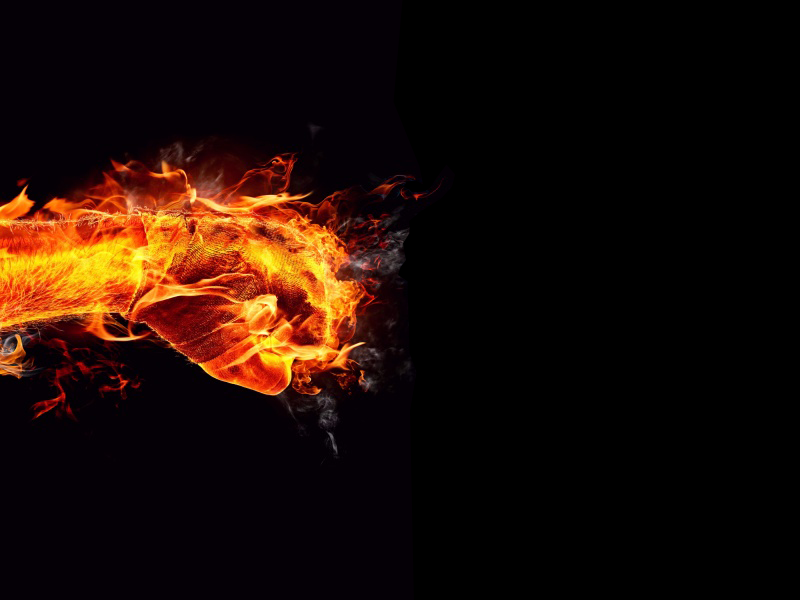
\includegraphics[scale=0.2]{arm1.png}
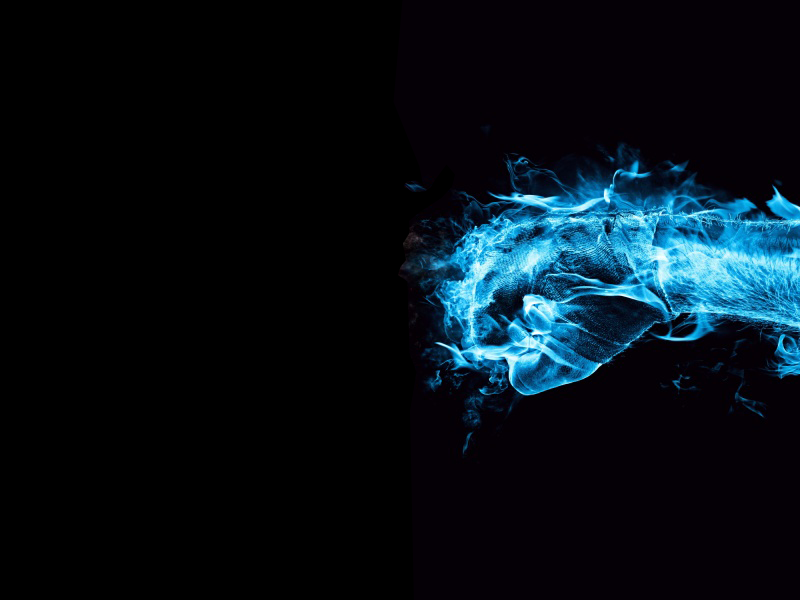
\includegraphics[scale=0.2]{arm2.png}
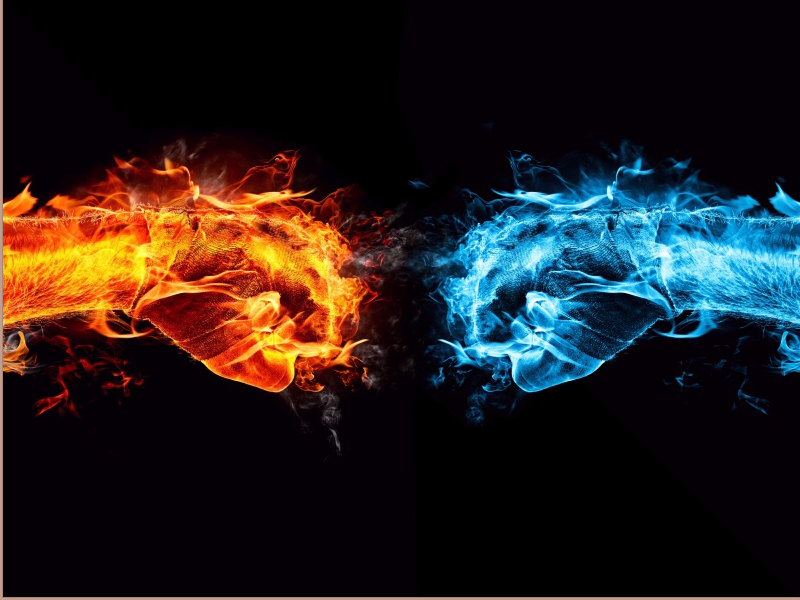
\includegraphics[scale=0.2]{arm-out.png}
\caption{arm1.png, arm2.png en arm-out.png}
\label{fig:Arm}
\end{figure}

\begin{figure}[h!]
\centering
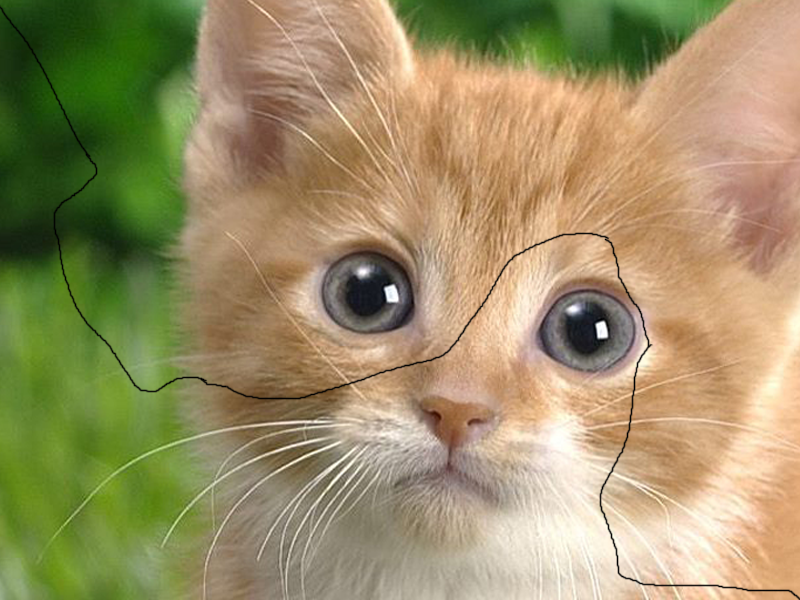
\includegraphics[scale=0.2]{animal1.png}
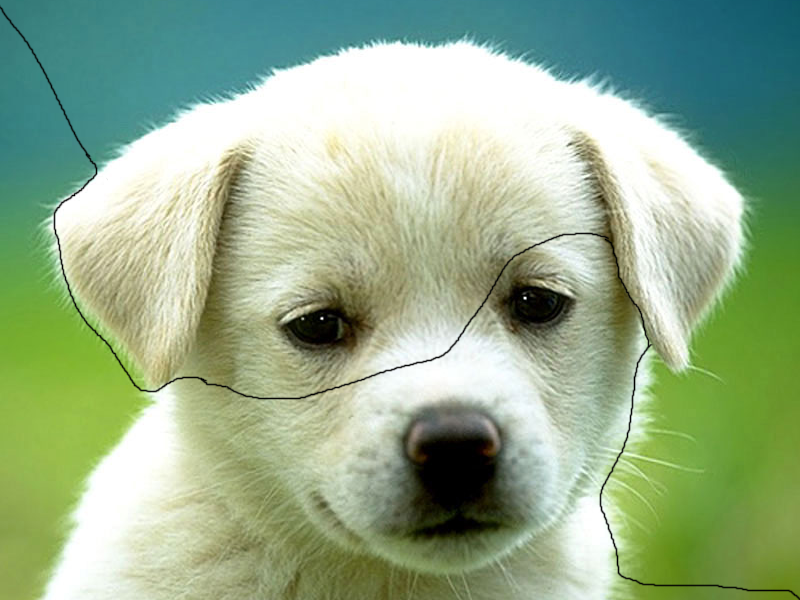
\includegraphics[scale=0.2]{animal2.png}
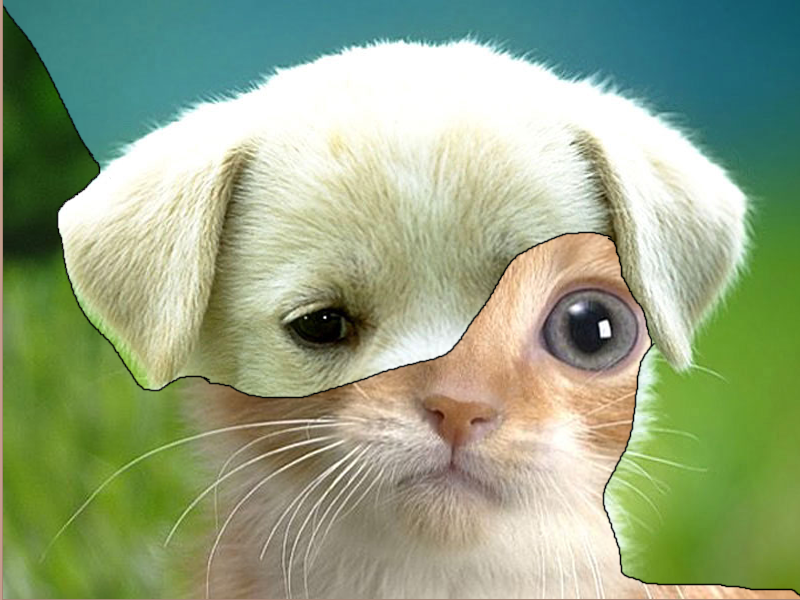
\includegraphics[scale=0.2]{animal-out.png}
\caption{animal1.png, animal2.png en animal-out.png}
\label{fig:Animal}
\end{figure}
\newpage


\bibliographystyle{nar}
\bibliography{references}
\end{document}
